%\section{Đề thi thử THPTQG Sở GD\&ĐT 25--26, Lần 1}

\caulc
\Opensolutionfile{ans}[ans/ans-59-26-2-HCM-ThanhDa-L1-LC]
\begin{ex}%[2D1N2-2]%[Lê Huỳnh Xuân Nguyên]
	Cho hàm số $y=f(x)$ có bảng biến thiên như bên dưới:
	\begin{center}
		
\begin{tikzpicture}
			\tkzTabInit[lgt=1.2,espcl=2]{$x$ /1.2, $f'(x)$ /1.2}{$-\infty$,$-3$,$0$,$8$,$+\infty$}
			\tkzTabLine{ ,-,z,+,z,-,z,+, }
		\end{tikzpicture}
	\end{center}
	Hỏi hàm số $y=f(x)$ có bao nhiêu điểm cực đại?
	\choice
	{$0$}
	{\True $1$}
	{$2$}
	{$3$}
	\loigiai{
		Ta có bảng biến thiên:
		\begin{center}
			\begin{tikzpicture}
				\tkzTabInit[lgt=1.2,espcl=2]{$x$ /1.2, $f'(x)$ /1.2, $f(x)$ /2.5}{$-\infty$,$-3$,$0$,$8$,$+\infty$}
				\tkzTabLine{ ,-,z,+,z,-,z,+, }
				\tkzTabVar{+/~ , -/ ~, +/ \text{CĐ}, -/~ , +/ ~}
			\end{tikzpicture}
		\end{center}
		Hàm số có một điểm cực đại duy nhất là $x = 0$.
	}
\end{ex}

\begin{ex}%[2D1N4-1]%[Lê Huỳnh Xuân Nguyên]
	Đồ thị hàm số $y=\dfrac{3-2x}{x+1}$ có tâm đối xứng là
	\choice
	{$I(-1;3)$}
	{\True $I(-1;-2)$}
	{$I(1;3)$}
	{$I(1;-2)$}
	\loigiai{
		Đồ thị hàm số có tiệm cận đứng $x = -\dfrac{d}{c} = -1$ và tiệm cận ngang $y = \dfrac{a}{c} = -2$.\\
		Do đó có tâm đối xứng là $I(-1;-2)$.
	}
\end{ex}

\begin{ex}%[2H2N1-2]%[Lê Huỳnh Xuân Nguyên]
	Cho hình hộp $ABCD.A'B'C'D'$. Tổng $\overrightarrow{BA'} + \overrightarrow{BC}$ bằng
	\begin{center}
		\begin{tikzpicture}[line join = round, line cap = round,>=stealth,scale=1]
			\coordinate (A) at (1,1);
			\coordinate (B) at (0,0);
			\coordinate (C) at (3,0);
			\coordinate (D) at ($(A)+(C)-(B)$);
			\coordinate (A') at (0.5,3);
			\coordinate (B') at ($(A')+(B)-(A)$);
			\coordinate (C') at ($(A')+(C)-(A)$);
			\coordinate (D') at ($(A')+(D)-(A)$);
			
			\draw [dashed] (B)--(A)--(D) (A)--(A');
			\draw (A')--(B')--(C')--(D')--cycle;
			\draw (B')--(B)--(C)--(C') (D')--(D)--(C);
			\draw [dashed, ->, thick] (B)--(A');
			\draw [->, thick] (B)--(C);
			
			\foreach \p/\pos in {A/left,B/left,C/right,D/right,A'/above,B'/left,C'/above,D'/above}
			\fill (\p) circle (1pt) node[\pos] {$\p$};
		\end{tikzpicture}
	\end{center}
	\choice
	{$\vec{BD}$}
	{\True $\vec{BD'}$}
	{$\vec{BC'}$}
	{$\vec{BB'}$}
	\loigiai{
		Vì $BCD'A'$ là hình bình hành nên $\overrightarrow{BA'} + \overrightarrow{BC} = \overrightarrow{BD'}$.
	}
\end{ex}
\begin{ex}%[2H5N1-3]%[Lê Huỳnh Xuân Nguyên]
	Trong không gian tọa độ $Oxyz,$ \;phương trình mặt phẳng đi qua ba điểm $A(3; 0; 0)$, $B(0; -1; 0)$ và $C(0; 0; 7)$ là
	\choice
	{\True $\dfrac{x}{3} - y + \dfrac{z}{7} = 1$}
	{$\dfrac{x}{3} - y + \dfrac{z}{7} = 0$}
	{$3x - y + 7z = 1$}
	{$3x - y + 7z = 0$}
	\loigiai{
		Áp dụng phương trình mặt phẳng theo đoạn chắn $\dfrac{x}{a} + \dfrac{y}{b} + \dfrac{z}{c} = 1$ ta có: 
		$$\dfrac{x}{3} + \dfrac{y}{-1} + \dfrac{z}{7} = 1 \Leftrightarrow \dfrac{x}{3} - y + \dfrac{z}{7} = 1.$$
	}
\end{ex}

\begin{ex}%[1D2N2-4]%[Lê Huỳnh Xuân Nguyên]
	Cho cấp số cộng $(u_n)$ có $u_1 = 3$ và công sai $d = 4$. Giá trị của $u_4$ bằng
	\choice
	{$11$}
	{$19$}
	{\True $15$}
	{$16$}
	\loigiai{
		Số hạng thứ $4$ của cấp số cộng là $u_4 = u_1 + 3d = 3 + 3 \cdot 4 = 15$.
	}
\end{ex}

\begin{ex}%[1D1N5-3]%[Lê Huỳnh Xuân Nguyên]
	Tất cả các nghiệm của phương trình $\sin x = \sin \dfrac{\pi}{5}$ là
	\choice
	{$x = \dfrac{\pi}{5} + k2\pi \ (k \in \mathbb{Z})$}
	{$x = -\dfrac{\pi}{5} + k2\pi \ (k \in \mathbb{Z})$}
	{\True $\hoac{&x = \dfrac{\pi}{5} + k2\pi \\ &x = \dfrac{4\pi}{5} + k2\pi} \ (k \in \mathbb{Z})$}
	{$\hoac{&x = \dfrac{\pi}{5} + k2\pi \\ &x = -\dfrac{\pi}{5} + k2\pi} \ (k \in \mathbb{Z})$}
	\loigiai{
		Phương trình $\sin x = \sin \alpha \Leftrightarrow \hoac{&x = \alpha + k2\pi \\ &x = \pi - \alpha + k2\pi} \ (k \in \mathbb{Z})$.\\
		Với $\alpha = \dfrac{\pi}{5}$, ta có $\pi - \dfrac{\pi}{5} = \dfrac{4\pi}{5}$.\\
		Vậy nghiệm là $\hoac{&x = \dfrac{\pi}{5} + k2\pi \\ &x = \dfrac{4\pi}{5} + k2\pi} \ (k \in \mathbb{Z})$.
	}
\end{ex}


\begin{ex}%[1D6N4-3]%[Lê Huỳnh Xuân Nguyên]
	Số nghiệm nguyên của bất phương trình $\log_2(x-1) \le 1$ là
	\choice
	{$1$}
	{$4$}
	{$3$}
	{\True $2$}
	\loigiai{
		Điều kiện $x - 1 > 0 \Leftrightarrow x > 1$.\\
		 Khi đó bất phương trình tương đương: $x - 1 \le 2^1 \Leftrightarrow x \le 3$.\\
		So điều kiện ta có nghiệm của bất phương trình là $1 < x \le 3$.\\
		Vì $x$ nguyên nên $x \in \{2; 3\}$. Vậy bất phương trình có $2$ nghiệm nguyên.
	}
\end{ex}
\begin{ex}%[1H8N4-2]%[Lê Huỳnh Xuân Nguyên]
	Cho hình chóp $S.ABCD$ có đáy $ABCD$ là hình vuông và $SA \perp (ABCD)$. Khẳng định nào sau đây \textbf{sai}?
	\choice
	{$(SAC) \perp (SBD)$}
	{$(SAC) \perp (ABCD)$}
	{$(SBC) \perp (SAB)$}
	{\True $(SBC) \perp (SCD)$}
	\loigiai{
		\begin{center}
			\begin{tikzpicture}
				\def\a{4}
				\def\h{4}
				\path 	(0:0) coordinate (A)
				++(0:\a) coordinate (D)
				++(-130:\a/2) coordinate (C)
				($(A)+(C)-(D)$) coordinate (B)
				($(A)+(90:\h)$) coordinate (S)
				(intersection of A--C and B--D) coordinate (O);%giao điểm O
				\draw[dashed,thick] 	(B)--(A)--(D)	(A)--(S);
				\draw[thick] 			(B)-- (C)--(D)
				(B)--(S)	(C)--(S)	(D)--(S);
				\foreach \x/\g in {A/135,B/-135,C/-45,D/45,S/90}
				\fill[black] 	(\x) circle (1.5pt)
				($(\g:3mm)+(\x)$) node {$\x$};	
				\draw pic[draw,angle radius=3mm]{right angle=D--A--S};%Theo chiều dương	
			\end{tikzpicture}
		\end{center}
		\begin{enumerate}
			\item Vì $\begin{cases} BD \perp AC \\ BD \perp SA \end{cases}$ nên $BD \perp (SAC) \Rightarrow (SBD) \perp (SAC)$.
			\item Vì $SA \perp (ABCD)$ nên $(SAC) \perp (ABCD)$.
			\item Vì $\begin{cases} BC \perp AB \\ BC \perp SA \end{cases}$ nên $BC \perp (SAB) \Rightarrow (SBC) \perp (SAB)$.
		\end{enumerate}
	}
\end{ex}

\begin{ex}%[1H8N7-1]%[Lê Huỳnh Xuân Nguyên]
	Thể tích của khối lăng trụ có diện tích đáy bằng $6$ và chiều cao bằng $4$ là
	\choice
	{$8$}
	{\True $24$}
	{$10$}
	{$12$}
	\loigiai{
		Thể tích khối lăng trụ $V = h \cdot S = 4 \cdot 6 = 24$.
	}
\end{ex}

\begin{ex}%[2D4H1-4]%[Lê Huỳnh Xuân Nguyên]
	$\displaystyle \int 2^x \cdot 5^x \, \mathrm{d}x$ bằng
	\choice
	{$\dfrac{2^x}{\ln 2} \cdot \dfrac{5^x}{\ln 5} + C$}
	{\True $\dfrac{10^x}{\ln 10} + C$}
	{$10^x \cdot \ln 10 + C$}
	{$\dfrac{2^x}{\ln 2} + \dfrac{5^x}{\ln 5} + C$}
	\loigiai{
		Ta có $\displaystyle \int 2^x \cdot 5^x \, \mathrm{d}x = \int (2 \cdot 5)^x \, \mathrm{d}x = \int 10^x \, \mathrm{d}x = \dfrac{10^x}{\ln 10} + C$.
	}
\end{ex}

\begin{ex}%[2D4N2-4]%[Lê Huỳnh Xuân Nguyên]
	Thể tích của khối tròn xoay khi quay hình phẳng giới hạn bởi đồ thị hàm số $y = \sqrt{\mathrm{e}^x + 1}$, trục hoành, đường thẳng $x = 0$ và $x = 2$ quanh trục hoành bằng
	\choice
	{\True $\pi \left(\mathrm{e}^2 + 1 \right)$}
	{$\pi \left(\mathrm{e}^2 + 2 \right)$}
	{$\left(\mathrm{e}^2 + 1 \right)$}
	{$\left(\mathrm{e}^2 + 2 \right)$}
	\loigiai{
		Thể tích khối tròn xoay là:
		$$V = \pi \displaystyle \int_0^2 \left( \sqrt{\mathrm{e}^x + 1} \right)^2 \mathrm{\,d}x = \pi \displaystyle \int_0^2 (\mathrm{e}^x + 1) \mathrm{\,d}x = \pi (\mathrm{e}^x + x)\Big|_0^2 = \pi \left(\mathrm{e}^2 + 1 \right).$$
	}
\end{ex}

\begin{ex}%[2D3H2-2]%[Lê Huỳnh Xuân Nguyên]
	Biểu đồ trong hình vẽ thể hiện điểm kiểm tra học kỳ 2 môn Toán của $501$ học sinh khối 12 của một trường THPT. Phương sai của mẫu số liệu ghép nhóm cho bởi biểu đồ này bằng bao nhiêu (kết quả làm tròn đến hàng phần trăm)?
	\begin{center}
		\begin{tikzpicture}[line join = round, line cap = round, >=stealth, scale=1]
			\pgfmathsetmacro{\w}{0.6} 
			\pgfmathsetmacro{\d}{0.4} 
			\pgfmathsetmacro{\v}{0.5/50} 
			
			% --- TRỤC TỌA ĐỘ ---
			\coordinate (O) at (0,0); 
			\draw[->] (O) -- (8,0) node[below left] {$\text{Điểm}$};
			\draw[->] (O) -- (0,3.2) node[above] {\text{Số hs}};
			
			% --- VẼ LƯỚI ---
			\foreach \y in {50,100,150,200,250}{
				\draw[gray!30, thin] (0,\y*\v) -- (7.2,\y*\v);
				\node[left] at (0,\y*\v) {\small \y};
			}
			
			% --- VẼ CỘT ---
			\foreach \txt / \val / \i in {{[4;5)}/25/0, {[5;6)}/50/1, {[6;7)}/102/2, {[7;8)}/202/3, {[8;9)}/112/4, {[9;10)}/10/5}{
				\pgfmathsetmacro{\xL}{0.5 + \i*(\w + \d)}
				\pgfmathsetmacro{\xR}{\xL + \w}
				\pgfmathsetmacro{\yH}{\val*\v}
				\draw[fill=black] (\xL,0) rectangle (\xR,\yH);
				\node[above] at ({(\xL+\xR)/2},\yH) {\footnotesize \val};
				\node[below] at ({(\xL+\xR)/2},0) {\footnotesize \txt};
			}
			\pgfresetboundingbox
			\path (O) (7.5,0) (0,3.5) (-0.8,-0.8);
		\end{tikzpicture}
	\end{center}
	\choice
	{$6$}
	{$1{,}13$}
	{\True $1{,}27$}
	{$1{,}49$}
	\loigiai{
		Số trung bình của mẫu số liệu ghép nhóm là:
		$$ \bar{x} = \frac{4{,}5 \cdot 25 + 5{,}5 \cdot 50 + 6{,}5 \cdot 102 + 7{,}5 \cdot 202 + 8{,}5 \cdot 112 + 9{,}5 \cdot 10}{501} = \frac{3612{,}5}{501} \approx 7{,}21 $$
		Phương sai của mẫu số liệu ghép nhóm là:
		$$ s^2 = \frac{1}{501} \left( 25 \cdot 4{,}5^2 + 50 \cdot 5{,}5^2 + 102 \cdot 6{,}5^2 + 202 \cdot 7{,}5^2 + 112 \cdot 8{,}5^2 + 10 \cdot 9{,}5^2 \right) - \left( \frac{3612{,}5}{501} \right)^2 $$
		$$ s^2 = \frac{26685{,}25}{501} - \left( \frac{3612{,}5}{501} \right)^2 \approx 1{,}2715 \dots $$
		Làm tròn kết quả đến hàng phần trăm, ta được phương sai $s^2 \approx 1{,}27$.
	}
\end{ex}
\Closesolutionfile{ans}


\cauds
\Opensolutionfile{ans}[ans/ans-59-26-2-HCM-ThanhDa-L1-DS]
\begin{ex}%[2D4V1-2]%[Lê Huỳnh Xuân Nguyên]
	Cây đậu Hà Lan khi trồng có chiều cao $3$ cm. Gọi $h(t)$ là độ cao tính bằng cm của cây đậu Hà Lan tại thời điểm $t$ kể từ khi được trồng, với $t$ tính theo tuần. Khảo sát cho thấy tốc độ tăng chiều cao của cây đậu Hà Lan sau khi trồng $t$ tuần là $h'(t) = -0{,}02t^3 + 0{,}3t^2$ (cm/tuần).
	\choiceTF
	{Hàm số $h(t)$ có công thức là $h(t) = -0{,}005t^4 + 0{,}1t^3$}
	{\True Giai đoạn tăng trưởng của cây đậu Hà Lan đó kéo dài $15$ tuần}
	{Chiều cao tối đa của cây đậu Hà Lan đó là $88$ cm}
	{\True Vào thời điểm cây đậu Hà Lan đó phát triển nhanh nhất thì chiều cao của cây là $53$ cm}
	\loigiai{
		\begin{itemchoice}
			\itemch \textbf{Sai.} Ta có $h(t) = \displaystyle \int h'(t)\mathrm{\,d}t = -0{,}005t^4 + 0{,}1t^3 + C$.\\
			Vì $h(0) = 3$ nên $-0{,}005 \cdot 0^4 + 0{,}1 \cdot 0^3 + C = 3 \Leftrightarrow C = 3$.\\
			Vậy $h(t) = -0{,}005t^4 + 0{,}1t^3 + 3$ (cm).
			\itemch \textbf{Đúng.} Xét bất phương trình $h'(t) \ge 0 \Leftrightarrow -0{,}02t^3 + 0{,}3t^2 \ge 0 \Leftrightarrow 0 \le t \le 15$ (vì $t \ge 0$).\\
			Vậy giai đoạn tăng trưởng của cây đậu Hà Lan kéo dài $15$ tuần.
			\itemch \textbf{Sai.} Cho $h'(t) = 0 \Leftrightarrow \left[\begin{aligned} &t=0 \\ &t=15 \end{aligned}\right.$\\
			Bảng biến thiên:
			\begin{center}
				
\begin{tikzpicture}
					\tkzTabInit[lgt=2, espcl=4, deltacl=0.8]{$t$ /1.2, $h'(t)$ /1.2, $h(t)$ /2.5}{$0$,$15$}
					\tkzTabLine{ ,+, }
					\tkzTabVar{-/ $3$, +/ $87{,}375$}
				\end{tikzpicture}
			\end{center}
			Vậy chiều cao tối đa của cây đậu Hà Lan là $87{,}375$ cm.
			\itemch \textbf{Đúng.} Ta có $h''(t) = -0{,}06t^2 + 0{,}6t$. Cho $h''(t) = 0 \Leftrightarrow \left[\begin{aligned} &t=0 \\ &t=10 \end{aligned}\right.$\\
			Bảng biến thiên:
			\begin{center}
				
\begin{tikzpicture}
					\tkzTabInit[lgt=1.2,espcl=2]{$t$ /1.2, $h''(t)$ /1.2, $h'(t)$ /2.5}{$0$,$10$,$15$}
					\tkzTabLine{ ,+,z,-, }
					\tkzTabVar{-/ , +/ , -/ }
				\end{tikzpicture}
			\end{center}
			Dựa vào bảng biến thiên, tốc độ tăng trưởng $h'(t)$ đạt cực đại tại $t=10$. Khi đó chiều cao của cây là $h(10) = -0{,}005 \cdot 10^4 + 0{,}1 \cdot 10^3 + 3 = 53$ (cm).
		\end{itemchoice}
	}
\end{ex}
\begin{ex}%[0D0V2-4]%[Lê Huỳnh Xuân Nguyên]
	Xét phép thử: Xếp ngẫu nhiên $9$ học sinh gồm $5$ nam, $4$ nữ thành một hàng dọc.
	\choiceTF
	{\True Số phần tử của không gian mẫu là bằng $9!$}
	{Xác suất để nam và nữ xếp xen kẽ bằng $\dfrac{1}{63}$}
	{Xác suất để nam xếp cạnh nhau và nữ xếp cạnh nhau bằng $\dfrac{1}{126}$}
	{\True Xác suất để $2$ học sinh nữ bất kỳ không đứng cạnh nhau bằng $\dfrac{5}{42}$}
	\loigiai{
		\begin{itemchoice}
			\itemch \textbf{Đúng.} Số phần tử của không gian mẫu là $n(\Omega) = 9!$.
			\itemch \textbf{Sai.} Gọi $A$ là biến cố: "Nam và nữ xếp xen kẽ".\\
			Vì có $5$ nam và $4$ nữ nên để xếp xen kẽ, các học sinh nam phải ở các vị trí lẻ, học sinh nữ ở các vị trí chẵn: $\text{Nam - Nữ - Nam - Nữ - Nam - Nữ - Nam - Nữ - Nam}$.\\
			Số cách xếp là $n(A) = 5! \cdot 4!$.\\
			Vậy xác suất $\mathrm{P}(A) = \dfrac{n(A)}{n(\Omega)} = \dfrac{5! \cdot 4!}{9!} = \dfrac{1}{126}$.
			\itemch \textbf{Sai.} Gọi $B$ là biến cố: "Nam xếp cạnh nhau và nữ xếp cạnh nhau".\\
			Ta nhóm $5$ học sinh nam thành nhóm $X$ và $4$ học sinh nữ thành nhóm $Y$.
			\begin{itemize}
				\item Bước 1: Xếp vị trí cho nhóm $X$ và $Y$ có $2!$ cách.
				\item Bước 2: Xếp chỗ cho $5$ học sinh nam trong nhóm $X$ có $5!$ cách.
				\item Bước 3: Xếp chỗ cho $4$ học sinh nữ trong nhóm $Y$ có $4!$ cách.
			\end{itemize}
			Theo quy tắc nhân $n(B) = 2! \cdot 5! \cdot 4!$. Vậy xác suất $\mathrm{P}(B) = \dfrac{n(B)}{n(\Omega)} = \dfrac{2! \cdot 5! \cdot 4!}{9!} = \dfrac{1}{63}$.
			\itemch \textbf{Đúng.} Gọi $C$ là biến cố: "2 học sinh nữ bất kỳ không đứng cạnh nhau".
			\begin{itemize}
				\item Bước 1: Xếp $5$ học sinh nam thành một hàng dọc có $5!$ cách.
				\item Bước 2: Giữa $5$ nam có $4$ khoảng trống và $2$ khoảng trống ở hai đầu, tổng là $6$ khoảng trống. Ta xếp $4$ học sinh nữ vào $6$ khoảng trống đó có $\mathrm{A}_6^4$ cách.
			\end{itemize}
			Theo quy tắc nhân $n(C) = 5! \cdot \mathrm{A}_6^4$. Vậy xác suất $\mathrm{P}(C) = \dfrac{5! \cdot \mathrm{A}_6^4}{9!} = \dfrac{5}{42}$.
		\end{itemchoice}
	}
\end{ex}
\begin{ex}%[2H5V3-4]%[Lê Huỳnh Xuân Nguyên]
	Trong không gian $Oxyz$ (đơn vị trên mỗi trục là $1$ mét), coi một phần mặt biển được khảo sát là mặt phẳng $(Oxy)$, trục $Oz$ hướng lên trên vuông góc với mặt biển, đỉnh của một ngọn hải đăng ở vị trí $I(21; 35; 50)$ cao $50$ mét so với mực nước biển và ngọn hải đăng này được thiết kế với vùng phủ sáng có bán kính là $4$ km. Một người đi biển ở vị trí $A(5\,121; 658; 0)$.
	\choiceTF
	{Phương trình mặt cầu mô tả ranh giới của vùng phủ sáng trên biển của ngọn hải đăng là $(x-21)^2 + (y-35)^2 + (z-50)^2 = 16$}
	{Người đi biển đang ở trong vùng phủ sáng của ngọn hải đăng}
	{\True Ngọn hải đăng phủ một vùng sáng trên mặt biển thì bán kính vùng phủ sáng này là $3\,999,7$ mét (làm tròn kết quả đến hàng phần mười, giả sử yếu tố bị che khuất bởi địa hình là không đáng kể)}
	{\True Giả sử người đi biển di chuyển theo đường thẳng đến chân ngọn hải đăng với tốc độ $7$ hải lí/giờ thì mất $5,27$ phút (làm tròn kết quả đến hàng phần trăm) để đến điểm đầu tiên ở trong vùng phủ sáng ngọn hải đăng trên. Biết $1$ hải lí $= 1\,852$ mét}
	
	\loigiai{
		\begin{center}
			\begin{tikzpicture}[
				declare function={
					r=2.;          % Bán kính mặt cầu
					tiso=0.3;       % Độ dẹt elip
					h=-1.0;         % Độ cao tâm cầu I so với mặt biển H
					rn=sqrt(r^2-h^2); % Bán kính vùng phủ sáng HF
					rny=tiso*rn;    % Trục dọc elip vùng sáng
				},
				line join=round, line cap=round, >=stealth, font=\footnotesize,
				intersect/node/.style={circle, fill, inner sep=1.2pt} 
				]
				
				% 1. Định nghĩa các điểm chính
				\coordinate (I) at (0,0);
				\coordinate (H) at (0,h);
				\coordinate (F) at (rn,h);
				\coordinate (A) at (-4,h-0.3);
				
				% 2. Vẽ mặt phẳng (Oxy) góc trái
				\begin{scope}[shift={(-5,h-0.8)}]
					\draw (-1,0) -- (2,0);
					\draw (-1,0) -- (2,1.2);
					\draw (0.7,0) arc (0:82:0.5);
					\node at (0.1,0.15) {$(Oxy)$};
				\end{scope}
				
				% 3. Vẽ khối cầu
				\draw (I) circle (r);
				\draw[gray!30, dashed] (180:r) arc (180:0:r and r*tiso);
				\draw[gray!30] (180:r) arc (180:360:r and r*tiso);
				
				% 4. Vẽ vùng phủ sáng và ĐẶT TÊN PATH để tính giao điểm
				\draw[dashed] ($(rn,h)$) arc (0:180:rn and rny); % Cung sau
				\path[name path=elip_truoc, thick] ($(rn,h)$) arc (0:-180:rn and rny); % Cung trước (dùng path để tính)
				\draw[thick] ($(rn,h)$) arc (0:-180:rn and rny); % Vẽ cung trước
				
				% 5. Xác định đường thẳng HA để tính giao điểm
				\path[name path=duong_HA] (H) -- (A);
				
				% 6. Tìm giao điểm K
				\path[name intersections={of=elip_truoc and duong_HA, by=K}];
				
				% 7. Vẽ các đoạn thẳng
				\draw[dashed] (I)--(H) (H)--(F) (I)--(F) node[midway,sloped,above]{4000};
				
				% Vẽ AH qua K 
				\draw (A) -- (K);
				\draw[red, dotted, thick] (K) -- (H);
				
				% Ký hiệu vuông góc
				\draw (H) ++(0,0.2) -- ++(0.2,0) -- ++(0,-0.2);
				
				% 8. Đổ điểm và nhãn
				\foreach \p/\pos in {I/above, H/below, F/right, A/left}
				\fill (\p) circle (1.2pt) node[\pos] {$\p$};
				\fill (K) circle (1.2pt) node[above left] {$K$};
				
			\end{tikzpicture}
		\end{center}
		\begin{itemchoice}
			\itemch \textbf{Sai.} Bán kính vùng phủ sáng $R = 4$ km $= 4\,000$ m. \\
			Phương trình mặt cầu là: $(x-21)^2 + (y-35)^2 + (z-50)^2 = 4\,000^2$.
			\itemch \textbf{Sai.}  Có:
			\begin{eqnarray*}
				IA = \sqrt{(5\,121-21)^2 + (658-35)^2 + (0-50)^2} = \sqrt{5\,100^2 + 623^2 + (-50)^2} \approx 5\,138
			\end{eqnarray*}
			Vì $ IA > 4\,000$ nên người đi biển ở vị trí $A$ thì nằm ngoài vùng phủ sáng.
			\itemch \textbf{Đúng.} Gọi $H$ là hình chiếu vuông góc của $I$ trên mặt biển $(Oxy)$. Ta có $H(21; 35; 0)$.\\
			Do đó $IH = \sqrt{0^2 + 0^2 + (-50)^2} = 50$.\\
			Xét $\triangle IHF$ vuông tại $H$: $HF = \sqrt{IF^2 - IH^2} = \sqrt{4\,000^2 - 50^2} \approx 3\,999{,}7$ (mét).
			\itemch \textbf{Đúng.} Gọi $K$ là điểm đầu tiên ở trong vùng phủ sáng.\\
			Có $AH = \sqrt{(5\,121-21)^2 + (658-35)^2} = \sqrt{5\,100^2 + 623^2} \approx 5\,138$.\\
			Khoảng cách cần di chuyển $AK = AH - HF \approx 5\,138 - 3\,999{,}7 \approx 1\,138{,}3$ (mét).\\
			Vận tốc $v = 7 \times 1\,852 = 12\,964$ (mét/giờ).\\
			Thời gian di chuyển $t = \dfrac{1\,138,3}{12\,964} \times 60 \approx 5{,}27$ (phút).
		\end{itemchoice}
	}
\end{ex}

\begin{ex}%[2D4V3-5]%[Lê Huỳnh Xuân Nguyên]
	Có một cái chòi hình "chóp cong", trong đó mái chòi $(H)$ có dạng hình "chóp lục giác cong đều" như hình vẽ bên dưới. Đáy của $(H)$ là một hình lục giác đều tâm $O$, đường chéo qua tâm $O$ có độ dài là $10$ m, chiều cao $SO = 10$ m ($SO$ vuông góc với mặt phẳng đáy). Các cạnh bên của $(H)$ là các sợi dây thép nằm trên các đường parabol có trục đối xứng song song với $SO$. Giả sử hình tạo bởi các đoạn giao tuyến của $(H)$ với mặt phẳng $(\alpha)$ vuông góc với $SO$ là một lục giác đều. Biết rằng khi mặt phẳng $(\alpha)$ đi qua trung điểm của $SO$ thì lục giác đều có cạnh $l = 2$ m.
\begin{center}
	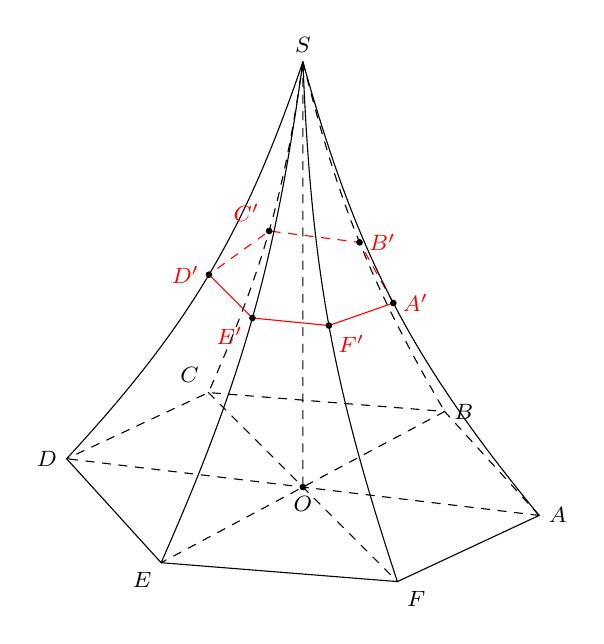
\begin{tikzpicture}[scale=1.2, font=\footnotesize, line join=round, line cap=round]
		% GÁN ĐIỂM S, A,B,...., F
		\coordinate (O) at (0,0);
		\coordinate (S) at (0,4.5);
		\coordinate (A) at (2.5, -0.3);  \coordinate (B) at (1.5, 0.8);
		\coordinate (C) at (-1.0, 1.0);  \coordinate (D) at (-2.5, 0.3);
		\coordinate (E) at (-1.5, -0.8); \coordinate (F) at (1.0, -1.0);
		
		% GÁN ĐIỂM A',B',...., F'
		\path (S) to[bend right=12] coordinate[pos=0.5] (A') (A);
		\path (S) to[bend right=8]  coordinate[pos=0.5] (B') (B);
		\path (S) to[bend left=8]   coordinate[pos=0.5] (C') (C);
		\path (S) to[bend left=12]  coordinate[pos=0.5] (D') (D);
		\path (S) to[bend left=8]   coordinate[pos=0.5] (E') (E);
		\path (S) to[bend right=8]  coordinate[pos=0.5] (F') (F);
		
		% 3. Vẽ nét khuất (Nét đứt) 
		\draw[dashed] (A)--(B)--(C)--(D) (A)--(D) (B)--(E) (C)--(F) (S)--(O);
		\draw[dashed] (S) to[bend right=8] (B) (S) to[bend left=8] (C);
		\draw[dashed, red] (A')--(B')--(C')--(D');
		
		% 4. Vẽ nét thấy (Nét liền) 
		\draw (D)--(E)--(F)--(A);
		\draw (S) to[bend right=12] (A) (S) to[bend left=12] (D) (S) to[bend left=8] (E) (S) to[bend right=8] (F);
		\draw[red] (D')--(E')--(F')--(A');
		
		% 5. Kí hiệu điểm
		\fill (O) circle (1pt) node[below] {$O$};
		\node[above] at (S) {$S$};
		\foreach \p/\pos in {A/right, B/right, C/above left, D/left, E/below left, F/below right} {
			\node[\pos] at (\p) {$\p$};
			\fill (\p') circle (1pt);
			\node[\pos, red] at (\p') {$\p'$};
		}
	\end{tikzpicture}
\end{center}
	\choiceTF
	{\True Diện tích hình lục giác đều nói trên khi $(\alpha)$ đi qua trung điểm của $SO$ là $6\sqrt{3}$ m$^2$}
	{\True Chọn hệ trục tọa độ $Oxy$ sao cho gốc tọa độ là điểm $O$ trên hình vẽ, $S$ thuộc tia $Oy$, đỉnh $A$ của lục giác đều thuộc tia $Ox$ thì parabol $(P)$ chứa cạnh bên $SA$ có phương trình $y = \dfrac{1}{6}x^2 - \dfrac{17}{6}x + 10$}
	{Nếu $(\alpha)$ cắt $SO$ và $(P)$ lần lượt tại $M$ và $B$, mà $OM = t$ thì độ dài đoạn $BM$ là $\dfrac{17}{2} - \sqrt{t + \dfrac{49}{4}}$}
	{\True Thể tích (m$^3$) phần không gian nằm bên trong mái chòi $(H)$ (làm tròn đến hàng phần mười) là $171,4$ m$^3$}
	\loigiai{
		
		\begin{itemchoice}
			
			\immini{
				\itemch \textbf{Đúng.} Diện tích của lục giác đều cạnh $2$ m bằng $6$ lần diện tích của tam giác đều cạnh bằng $2$ m nên:
				\begin{eqnarray*}
					S = 6 \cdot \dfrac{2^2 \cdot \sqrt{3}}{4} = 6\sqrt{3} \text{ (m}^2\text{)}.
				\end{eqnarray*}		
				\itemch \textbf{Đúng.} 
			$(P) : y = ax^2 + bx + c$ đi qua $A(5; 0)$, $S(0; 10)$, $A'(2; 5)$ nên:\\
			$ \begin{cases} 
				25a + 5b + c = 0 \\ 
				0a + 0b + c = 10 \\ 
				4a + 2b + c = 5 
			\end{cases} \Leftrightarrow 
			\begin{cases} 
				a = \dfrac{1}{6} \\ 
				b = -\dfrac{17}{6} \\ 
				c = 10 
			\end{cases}.$}{
		\begin{tikzpicture}[>=stealth, scale=0.6, font=\footnotesize]
			\draw[->] (-1,0) -- (8,0) node[below] {$x$};
			\draw[->] (0,-1) -- (0,11) node[left] {$y$};
			\node[below left] at (0,0) {$O$};
			
			\draw[thick, blue, samples=100, domain=0:5] plot (\x, {1/6*(\x)^2 - 17/6*\x + 10});
			
			\def\t{1.8} % Giá trị t mẫu
			\draw[thick, red] (-1,\t) -- (6,\t) node[right] {$y = t$};
			
			\coordinate (S) at (0,10);
			\coordinate (A) at (5,0);
			\coordinate (A1) at (2,5);
			\coordinate (M) at (0,\t);
			\coordinate (B) at (3.57,\t); % Giao điểm của y=t và Parabol
			
			\draw[dashed] (2,0) -- (2,5) node [above right] {$ A' $} -- (0,5);
			\node[left] at (0,5) {$5$};
			\node[below] at (2,0) {$2$};
			\node[left] at (0,10) {$10$};
			\node[below] at (5,0) {$5$};
			
			\node[red, above left] at (M) {$M$};
			\node[red, above right] at (B) {$B$};
			
		\end{tikzpicture}
		}
			
			\itemch \textbf{Sai.}Đường thẳng $y = t$ ($0 \le t \le 10$) cắt $Oy$, $(P)$ lần lượt tại $M$, $B$. Khi đó độ dài đoạn $MB = x_B < 5$.\\
			Xét phương trình 
			\begin{eqnarray*}
				t = \frac{1}{6}x^2 - \frac{17}{6}x + 10 \Leftrightarrow x^2 - 17x + 60 - 6t = 0 \Leftrightarrow x = \frac{17 \pm \sqrt{24t + 49}}{2}
			\end{eqnarray*}
			Vì $MB < 5$ nên $MB = \dfrac{17 - \sqrt{24t + 49}}{2} = \dfrac{17}{2} - \sqrt{6t + \dfrac{49}{4}}$.
			
			\itemch \textbf{Đúng.} Diện tích thiết diện cắt $SO$ tại $M$ là: 
			\begin{eqnarray*}
				S(t) = 6 \cdot \frac{MB^2\sqrt{3}}{4} = \frac{3\sqrt{3}}{2} \left( \frac{17}{2} - \sqrt{6t + \frac{49}{4}} \right)^2
			\end{eqnarray*}
			Thể tích khối chóp lục giác cong đều là: 
			\begin{eqnarray*}
				V = \displaystyle\int\limits_{0}^{10} \frac{3\sqrt{3}}{2} \left( \frac{17}{2} - \sqrt{6t + \frac{49}{4}} \right)^2 \mathrm{\,d}t \approx 171{,}4 \text{ (m}^3\text{)}
			\end{eqnarray*}
		\end{itemchoice}
	}
\end{ex}
\Closesolutionfile{ans}

\caukq
\Opensolutionfile{ans}[ans/ans-59-26-2-HCM-ThanhDa-L1-KQ]
\begin{ex}%[2D1H3-6]%[Lê Huỳnh Xuân Nguyên]
	Một nhà máy sản xuất $x$ sản phẩm trong mỗi tháng. Chi phí sản xuất $x$ sản phẩm được cho bởi hàm chi phí $C(x) = 1\,600 + 500x - 1{,}6x^2 + 0{,}004x^3$ (nghìn đồng). Biết giá bán của mỗi sản phẩm là một hàm số phụ thuộc vào số lượng sản phẩm $x$ và được cho bởi công thức $p(x) = 1\,700 - 7x$ (nghìn đồng). Hỏi mỗi tháng nhà máy nên sản xuất bao nhiêu sản phẩm để lợi nhuận thu được là lớn nhất, biết rằng kết quả khảo sát thị trường cho thấy sản phẩm sản xuất ra sẽ được tiêu thụ hết?
	\shortans{100}
	\loigiai{
		Điều kiện: $\begin{cases} x \ge 0 \\ 1\,700 - 7x \ge 0 \end{cases} \Leftrightarrow 0 \le x \le \dfrac{1\,700}{7}$.\\
		Lợi nhuận thu được là:
		\begin{eqnarray*}
			&L(x) = x(1700 - 7x) - (1\,600 + 500x - 1{,}6x^2 + 0{,}004x^3) \\
			&L(x) = -0{,}004x^3 - 5{,}4x^2 + 1200x - 1600.
		\end{eqnarray*}
		\noindent Có $L'(x) = -0{,}012x^2 - 10{,}8x + 1\,200$.\\
		Cho $L'(x) = 0 \Leftrightarrow \hoac{ &x = 100 \text{ (nhận)} \\ &x = -1\,000 \text{ (loại)}.}$\\
		Bảng biến thiên:
		\begin{center}
			
\begin{tikzpicture}
				\tkzTabInit[lgt=1.2,espcl=3]{$x$ /1, $L'(x)$ /1, $L(x)$ /2}{0, 100, $\frac{1700}{7}$}
				\tkzTabLine{ , +, 0, -, }
				\tkzTabVar{-/ , +/ , -/ }
			\end{tikzpicture}
		\end{center}
		Vậy lợi nhuận thu được lớn nhất khi nhà máy sản xuất $100$ sản phẩm.
	}
\end{ex}
\begin{ex}%[1H8H5-4]%[Lê Huỳnh Xuân Nguyên]
	Cho hình chóp $S.ABCD$ có đáy $ABCD$ là hình vuông cạnh bằng $2$. Hình chiếu vuông góc của điểm $S$ lên mặt phẳng $(ABCD)$ trùng với trung điểm của cạnh $AB$. Biết $[S, AD, B] = 60^\circ$. Tính khoảng cách giữa hai đường thẳng $AB$ và $SC$ (làm tròn kết quả đến hàng phần trăm).
	\shortans{1{,}31}
	\loigiai{
		\begin{enumerate}
			\item[\textbf{Cách 1.}] Gán hệ tọa độ $Oxyz$.
			\immini{
				Ta có $\begin{cases} AD \perp AB \\ AD \perp SH \text{ (do } SH \perp (ABCD)) \end{cases}$\\
				 Do đó: $AD \perp (SAB) \Rightarrow AD \perp SA$. \\
				Mà $AB \perp AD$  \\
				Nên $[S, AD, B] = \widehat{SAB} = 60^\circ$. \\
				Chọn hệ trục tọa độ $Oxyz$ như hình vẽ. Khi đó ta có: $A(-1; 0; 0), B(1; 0; 0)$ và $C(1; 2; 0)$. 
			}{
				\begin{tikzpicture}[scale=0.7, font=\footnotesize, line join=round, line cap=round, >=stealth]
					\def\a{7}
					\def\h{6}
					\path (0:0) coordinate (A)    ++(0:\a) coordinate (D)    ++(-150:\a/2) coordinate (C) ($(A)+(C)-(D)$) coordinate (B)    ($(A)!0.5!(B)$) coordinate (H)    ($(H)+(90:\h)$) coordinate (S) (intersection of A--C and B--D) coordinate (O);%giao điểm O
					% --- VẼ HỆ TRỤC TỌA ĐỘ (MÀU ĐỎ) ---
					%  Vẽ các đường và mũi tên Ox, Oy, Oz
					\draw[->,red,thick] (S) -- ($(S)+(0,1.5)$); % Tia Oz
					\draw[->,red,thick] (B) -- ($(B)+($(B)-(H)$)$); % Tia Ox
					\draw[red,dashed,thick] (H) -- ++(0:\a); 
					\draw[->,red,thick] ($(H)+(0:\a)$) -- ($(H)+(0:\a)+(2,0)$); % Tia Oy kéo dài ra ngoài
					% node Ox, Oy, Oz
					\node[left,red] at ($(S)+(0,1.5)$) {$z$};
					\node[left,red] at ($(B)+($(B)-(H)$)$) {$x$};
					\node[above,red] at ($(H)+(0:\a)+(2,0)$) {$y$};
					% --- VẼ HÌNH CHÓP ---
					\draw[dashed,thick] (B)--(A)--(D) (A)--(S) (S)--(H) ;
					\draw[thick] (B)--(C)--(D) (B)--(S) (C)--(S) (D)--(S);
					% --- : KÝ HIỆU  GÓC ---
					% Vuông góc tại H 
					\draw ($(H)+(0,0.35)$) -- ($(H)+(0.25,0.45)$) -- ($(H)+(0.25,0.1)$);
					% Vuông góc tại A
					
					\draw (A)--++(0.4,0)--++(-150:0.4)--++(-0.4,0)--cycle;
					%				
					%				% Vuông góc tại D
					\draw (D)--++(-0.4,0)--++(-150:0.4)--++(0.4,0)--cycle;
					%				
					%				% Vuông góc tại B
					\draw (B)--++(30:0.4)--++(0.6,0)--++(-150:0.4)--cycle;
					%				
					%				% Vuông góc tại D
					\draw (C)--++(-0.5,0)--++(30:0.4)--++(0.5,0)--cycle;
					
					% ---  Ký hiệu góc SAB ---
					\draw ($(A)!0.7cm!(S)$) arc (115:220:0.55);
					\node at ($(A)+(-0.6,0.6)$) {$60^\circ$};
					
					% Vòng lặp hiển thị tên điểm
					\foreach \x/\g in {A/45,B/-135,C/-45,D/45,S/135,H/150}
					\fill[black] (\x) circle (1.5pt) ($(\g:4mm)+(\x)$) node {$\x$};
					
				\end{tikzpicture}
			}
			Ta có:
			\begin{eqnarray*}
				\tan 60^\circ = \dfrac{SH}{AH} \Rightarrow \sqrt{3} = \dfrac{SH}{1} \Rightarrow SH = \sqrt{3} \Rightarrow S(0; 0; \sqrt{3})
			\end{eqnarray*}
			Vậy $$\begin{cases} \overrightarrow{AB} = (2; 0; 0) \\ \overrightarrow{SC} = (1; 2; -\sqrt{3}) \\ \overrightarrow{AS} = (1; 0; \sqrt{3}) \end{cases}$$ 
			nên 
			\begin{eqnarray*}
				\mathrm{d}(AB, SC) = \dfrac{\left| \left[ \overrightarrow{AB}, \overrightarrow{SC} \right] \cdot \overrightarrow{AS} \right|}{\left| \left[ \overrightarrow{AB}, \overrightarrow{SC} \right] \right|} \approx 1{,}31
			\end{eqnarray*}
			\item[\textbf{Cách 2.}] Dùng hình học không gian thuần túy.
			\immini{
				\noindent
				* Vì $AB \parallel (SCD)$ nên ta có:
				$$\mathrm{d}(AB, SC) = \mathrm{d}(AB, (SCD)) = \mathrm{d}(H, (SCD)).$$
				* Vẽ $HE \perp CD$ tại $E$ ($E$ là trung điểm $CD$).\\
				Ta có $CD \perp (SHE) \Rightarrow CD \perp HF$.\\
				* Vẽ $HF \perp SE$ tại $F$. Ta có $HF \perp (SCD)$.\\
				Do đó $\mathrm{d}(H, (SCD)) = HF$.\\
				* Có $\dfrac{1}{HF^2} = \dfrac{1}{SH^2} + \dfrac{1}{HE^2} \Rightarrow HF \approx 1{,}31$.
			}{
				\begin{tikzpicture}[scale=0.7, font=\footnotesize, line join=round, line cap=round, >=stealth]
					\def\a{7}
					\def\h{6}
					\path (0:0) coordinate (A)    ++(0:\a) coordinate (D)    ++(-150:\a/2) coordinate (C) ($(A)+(C)-(D)$) coordinate (B)    ($(A)!0.5!(B)$) coordinate (H)    ($(H)+(90:\h)$) coordinate (S) (intersection of A--C and B--D) coordinate (O)($(C)!0.5!(D)$) coordinate (E)
					($(S)!0.377777!(E)$) coordinate (F);
					
					% --- VẼ TAM GIÁC SHE---
					\draw[dashed] (H)--(E) ;
					\draw (S)--(E) ;
					\draw[dashed,red,thick] (H)--(F);
					
					% --- VẼ HÌNH CHÓP ---
					\draw[dashed,thick] (B)--(A)--(D) (A)--(S) (S)--(H) ;
					\draw[thick] (B)--(C)--(D) (B)--(S) (C)--(S) (D)--(S);
					
					% --- : KÝ HIỆU GÓC ---
					% Vuông góc tại H 
					\draw ($(H)+(0,0.35)$) -- ($(H)+(0.25,0.45)$) -- ($(H)+(0.25,0.1)$);
					% Vuông góc tại A
					\draw (A)--++(0.4,0)--++(-150:0.4)--++(-0.4,0)--cycle;			
					% Vuông góc tại D
					\draw (D)--++(-0.4,0)--++(-150:0.4)--++(0.4,0)--cycle;			
					% Vuông góc tại B
					\draw (B)--++(30:0.4)--++(0.6,0)--++(-150:0.4)--cycle;				
					% Vuông góc tại C
					\draw (C)--++(-0.5,0)--++(30:0.4)--++(0.5,0)--cycle;
					
					% Ký hiệu vuông góc tại E (Thêm mới)
					\draw ($(E)!0.3cm!(C)$) -- ($($(E)!0.3cm!(C)$)+($(E)!0.3cm!(H)$)-(E)$) -- ($(E)!0.3cm!(H)$);
					
					% Ký hiệu vuông góc tại F (Thêm mới, màu đỏ)
					\draw[red, thick] ($(F)!0.3cm!(H)$) -- ($($(F)!0.3cm!(H)$)+($(F)!0.3cm!(S)$)-(F)$) -- ($(F)!0.3cm!(S)$);
					
					% ---  Ký hiệu góc SAB ---
					\draw ($(A)!0.7cm!(S)$) arc (115:220:0.55);
					\node at ($(A)+(-0.6,0.6)$) {$60^\circ$};
					
					% Vòng lặp hiển thị tên điểm
					\foreach \x/\g in {A/45,B/-135,C/-45,D/45,S/135,H/150,E/-50,F/0}
					\fill[black] (\x) circle (1.5pt) ($(\g:4mm)+(\x)$) node {$\x$};
					
				\end{tikzpicture}
			}
		\end{enumerate}
		
	}
\end{ex}

\begin{ex}%[0D2V2-3]%[Lê Huỳnh Xuân Nguyên]
	Bác Hai có một mảnh đất rộng $6$ héc-ta. Bác dự tính trồng cà chua và bắp cho mùa vụ sắp tới. Nếu trồng bắp thì bác Hai cần $10$ ngày để trồng một héc-ta. Nếu trồng cà chua thì bác Hai cần $20$ ngày để trồng một héc-ta. Biết rằng mỗi ha bắp sau thu hoạch bán được $30$ triệu đồng, mỗi héc-ta cà chua sau thu hoạch bán được $50$ triệu đồng và bác Hai chỉ còn $100$ ngày để canh tác cho kịp mùa vụ. Số tiền nhiều nhất mà bác Hai có thể thu được sau mùa vụ này là bao nhiêu triệu đồng?
	\shortans{260}
	\loigiai{
		\immini{
		Gọi $x, y$ lần lượt là số héc-ta trồng cà chua và bắp.
		
		Ta có hệ $\begin{cases} x \ge 0 \\ y \ge 0 \\ x + y \le 6 \\ 20x + 10y \le 100. \end{cases}$\\
		
		Miền nghiệm của hệ trên là miền đa giác $OABC$ với $O(0;0)$, $A(0;6)$, $B(4;2)$ và $C(5;0)$.\\
		Số tiền bác Hai thu được là: $T(x;y) = 50x + 30y$ (triệu đồng).\\
		Ta có: $T(0;0) = 0$; $T(0;6) = 180$; $T(4;2) = 260$; $T(5;0) = 250$.
		}{
		\begin{tikzpicture}[scale=0.5, font=\footnotesize, >=stealth]
			% --- 1. VẼ LƯỚI Ô VUÔNG ---
			\draw[gray!30, step=0.5] (-1,-1) grid (7,11);
			
			% --- 2. MIỀN NGHIỆM KHÔNG BỊ GẠCH (Đa giác OABC) ---
			\fill[gray!10] (0,0) -- (0,6) -- (4,2) -- (5,0) -- cycle;
			
			% --- 3. CÁC MIỀN GẠCH BỎ (DỌC VÀ NGANG) ---
			\pattern[pattern=vertical lines, pattern color=gray!60] (0,6) -- (4,2) -- (0,10) -- cycle;
			\pattern[pattern=horizontal lines, pattern color=gray!60] (0,10) -- (4,2) -- (5,0) -- (7,0) -- (7,11) -- (0,11) -- cycle;
			
			% Gạch sọc nền hệ trục cho x < 0 và y < 0
			\pattern[pattern=north west lines, pattern color=gray!50] (-1,-1) rectangle (0,11);
			\pattern[pattern=north west lines, pattern color=gray!50] (-1,-1) rectangle (7,0);
			\fill[pattern=north east lines, pattern color=gray!50] (4,2) -- (5,0) -- (6,0) -- cycle;
			
			% --- 4. VẼ CÁC ĐƯỜNG THẲNG GIỚI HẠN (Đã tách rời nhãn chữ) ---
			\draw[blue, thick, domain=-0.5:6.5] plot (\x, {6-\x});
			\node[blue, right] at (6.5, -0.5) {$x+y=6$};
			
			% Đường thẳng đỏ (nhãn đặt dịch hẳn lên phía trên đầu đường)
			\draw[red, thick, domain=-0.5:5.5] plot (\x, {10-2*\x});
			\node[red, above right] at (-0.5, 11) {$20x+10y=100$};
			
			% --- 5. VẼ HỆ TRỤC TỌA ĐỘ OXY ---
			\draw[->, thick] (-1,0) -- (7,0) node[below] {$x$};
			\draw[->, thick] (0,-1) -- (0,11) node[left] {$y$};
			\draw[dashed] (4,0) -- (4,2) -- (0,2);
			
			% --- 6. RÚT GỌN BẰNG FOREACH: HIỂN THỊ ĐIỂM VÀ NHÃN TỌA ĐỘ ---
			\foreach \coord/\pos/\label in {
				{0,0}/below left/O,
				{0,2}/left/2,
				{0,6}/left/A,
				{0,10}/left/10,
				{4,0}/below/4,
				{5,0}/below/C,
				{6,0}/below/6,
				{4,2}/above right/B
			} {
				\fill (\coord) circle (2pt);
				\node[\pos] at (\coord) {$\label$};
			}
		\end{tikzpicture}
		}
		\noindent Vậy số tiền nhiều nhất mà bác Hai có thể thu được là $260$ triệu đồng khi trồng $4$ héc-ta cà chua và $2$ héc-ta bắp.
	}
	
\end{ex}

\begin{ex}%[2H2V2-6]%[Lê Huỳnh Xuân Nguyên]
	Trong không gian với hệ trục tọa độ $Oxyz$ cho trước (đơn vị trên mỗi trục là km), một trạm kiểm soát hải quân phát hiện một chiếc tàu lạ ở vị trí $A(9; 12; 0)$ đang di chuyển theo hướng véc-tơ $\overrightarrow{v}_1 = (-3; 4; 0)$ với vận tốc $30$ km/h. Ngay lập tức, trạm kiểm soát điều khiển một máy bay không người lái đang ở vị trí $B(0; 0; 1)$ di chuyển theo hướng véc-tơ $\overrightarrow{v}_2 = (5; 12; 0)$ với vận tốc $130$ km/h để tiếp cận chiếc tàu lạ đó. Hỏi sau bao nhiêu phút thì khoảng cách giữa máy bay không người lái và chiếc tàu lạ đó ngắn nhất (làm tròn kết quả đến hàng phần trăm)?
	\shortans{7{,}65}
	\loigiai{
		Gọi $\overrightarrow{v}_A, \overrightarrow{v}_B$ lần lượt là véc-tơ vận tốc của chiếc tàu và máy bay.\\
		Ta có: 
		\begin{eqnarray*}
			\dfrac{\overrightarrow{v}_A}{30} = \dfrac{\overrightarrow{v}_1}{\sqrt{(-3)^2 + 4^2 + 0^2}} \Rightarrow \overrightarrow{v}_A = 6\overrightarrow{v}_1 \Rightarrow \overrightarrow{v}_A = (-18; 24; 0).
		\end{eqnarray*}
		Do đó vị trí $A'$ của chiếc tàu sau thời gian $t$ (giờ) là: $A'(9 - 18t; 12 + 24t; 0)$.\\
		Ta có: 
		\begin{eqnarray*}
			\dfrac{\overrightarrow{v}_B}{130} = \dfrac{\overrightarrow{v}_2}{\sqrt{5^2 + 12^2 + 0^2}} \Rightarrow \overrightarrow{v}_B = 10\overrightarrow{v}_2 \Rightarrow \overrightarrow{v}_B = (50; 120; 0)
		\end{eqnarray*}
		Do đó vị trí $B'$ của máy bay sau thời gian $t$ (giờ) là: $B'(50t; 120t; 1)$.\\
		Ta có: 
		\begin{eqnarray*}
			A'B' = \sqrt{(68t - 9)^2 + (96t - 12)^2 + 1^2} = \sqrt{13\,840t^2 - 3\,528t + 226}.
		\end{eqnarray*}
		Bảng biến thiên của hàm số $f(t) = 13\,840t^2 - 3\,528t + 226$
		\begin{center}
			
\begin{tikzpicture}
				\tkzTabInit[lgt=1.2,espcl=3.5]{$t$ /1, $f'(t)$ /1, $f(t)$ /2}{$0$, $\frac{441}{3460}$, $+\infty$}
				\tkzTabLine{ , -, 0, +, }
				\tkzTabVar{+/ , -/ $\text{min}$ , +/ }
			\end{tikzpicture}
		\end{center}
		Ta được $f(t)$ đạt giá trị nhỏ nhất tại 
		\begin{eqnarray*}
			t = \dfrac{3\,528}{2 \cdot 13\,840} \; \text{giờ }\approx 7{,}65 \; \text{phút.}
		\end{eqnarray*}
		Vậy sau khoảng $7{,}65$ phút thì khoảng cách giữa máy bay và tàu ngắn nhất.
	}
\end{ex}
\begin{ex}%[2D6V2-4]%[Lê Huỳnh Xuân Nguyên]
	Có hai chiếc hộp, hộp I có $5$ quả bóng đỏ và $3$ quả bóng vàng, hộp II có $4$ quả bóng đỏ và $6$ quả bóng vàng, các quả bóng có cùng kích thước và khối lượng. Lấy ngẫu nhiên một quả bóng từ hộp I rồi chuyển (bỏ) vào hộp II. Sau đó, lấy ra ngẫu nhiên hai quả bóng từ hộp II. Biết rằng trong hai quả bóng lấy ra từ hộp II có ít nhất một quả màu đỏ. Tính xác suất để quả bóng được chuyển từ hộp I sang là quả bóng màu đỏ (làm tròn kết quả đến hàng phần trăm).
	\shortans{0{,}66}.
	\loigiai{
	\begin{center}
		\begin{tikzpicture}[sloped, scale=0.85, font=\footnotesize]
			
			% Điểm gốc sơ đồ cây
			\node[draw, rectangle, inner sep=3pt] (Origin) at (0,0) {};
			
			% --- NHÁNH DƯỚI (Biến cố A_bar) ---
			\node (A_bar) at (4.5, -3) {$\overline{A}$: "Hộp I lấy $1$ bóng vàng"};
			
			% Con của nhánh dưới 
			\node (B_A_bar) at (15.5, -1) {$B$: "Hộp II lấy ít nhất $1$ quả đỏ"};
			\node (B_bar_A_bar) at (15.5, -5) {$\overline{B}$: "Hộp II không lấy quả đỏ nào"};
			
			% --- NHÁNH TRÊN (Biến cố A) ---
			\node (A) at (4.5, 3) {$A$: "Hộp I lấy $1$ bóng đỏ"};
			
			% Con của nhánh trên 
			\node (B_A) at (15.5, 5) {$B$: "Hộp II lấy ít nhất $1$ quả đỏ"};
			\node (B_bar_A) at (15.5, 1) {$\overline{B}$: "Hộp II không lấy quả đỏ nào"};
			
			% --- VẼ CÁC ĐƯỜNG NỐI VÀ GÁN XÁC SUẤT ---
			\draw[->] (Origin) -- node[above] {$\mathrm{P}(A) = \dfrac{5}{8}$} (A);
			\draw[->] (Origin) -- node[below] {$\mathrm{P}(\overline{A}) = \dfrac{3}{8}$} (A_bar);
			
			% Node biến cố
			\draw[->] (A) -- node[above] {$\mathrm{P}(B|A) = 1 - \dfrac{3}{11} = \dfrac{8}{11}$} (B_A);
			\draw[->] (A) -- node[below] {$\mathrm{P}(\overline{B}|A) = \dfrac{\mathrm{C}_6^2}{\mathrm{C}_{11}^2} = \dfrac{3}{11}$} (B_bar_A);
			
			\draw[->] (A_bar) -- node[above] {$\mathrm{P}(B|\overline{A}) = 1 - \dfrac{21}{55} = \dfrac{34}{55}$} (B_A_bar);
			\draw[->] (A_bar) -- node[below] {$\mathrm{P}(\overline{B}|\overline{A}) = \dfrac{\mathrm{C}_7^2}{\mathrm{C}_{11}^2} = \dfrac{21}{55}$} (B_bar_A_bar);
			
		\end{tikzpicture}
	\end{center}
		\vspace{0.3cm}
		Ta có:
		\begin{eqnarray*}
			\mathrm{P}(A|B) = \dfrac{\mathrm{P}(B|A) \cdot \mathrm{P}(A)}{\mathrm{P}(B)} = \dfrac{\dfrac{8}{11} \cdot \dfrac{5}{8}}{\dfrac{5}{8} \cdot \dfrac{8}{11} + \dfrac{3}{8} \cdot \dfrac{34}{55}} \approx 0{,}66.
		\end{eqnarray*}
	}
\end{ex}

\begin{ex}%[2H2V2-6]%[Lê Huỳnh Xuân Nguyên]
	Nhân ngày Khai giảng năm học mới, các chú bảo vệ của trường THPT A dùng dây thừng có gắn đủ màu sắc để trang trí. Trong không gian $Oxyz$, mỗi đơn vị trên trục tọa độ là mét, mặt phẳng $Oxy$ là mặt đất, trục $Oz$ hướng lên trời. Có ba cây cột được cắm trên sân trường, trong đó:
	\begin{itemize}
		\item Chân của cột 1 (chiều cao $10$ m) nằm ở gốc tọa độ;
		\item Chân của cột 2 (chiều cao $15$ m) nằm trên trục $Ox$;
		\item Chân của cột 3 (chiều cao $20$ m) nằm trên trục $Oy$;
		\item Khoảng cách từ cột 1 đến cột 2 là $30$ m và khoảng cách từ cột 2 đến cột 3 là $50$ m.
	\end{itemize}
	Để trang trí cho ngày lễ, chú bảo vệ sẽ:
	\begin{itemize}
		\item Nối dây từ đỉnh cột 2 xuống mặt đất rồi lại nối lên đỉnh cột 1;
		\item Từ đỉnh cột 1 kéo dây nối xuống mặt đất rồi tiếp lên đỉnh cột 3.
	\end{itemize}
	\immini{
	Gọi $A(x; y; z)$ và $B(a; b; c)$ là hai vị trí chạm đất của dây thừng. Gọi $T$ là tổng chiều dài sợi dây ngắn nhất sau khi nối từ đỉnh cột 2 đến đỉnh cột 3. Tính giá trị $x + y + z + a + b + c + T$ (Không làm tròn các giá trị trung gian, chỉ làm tròn kết quả cuối cùng đến hàng đơn vị).
	}{
	\begin{tikzpicture}[scale=0.7, font=\normalsize, >=stealth]
		% --- 1. Định nghĩa tọa độ các điểm ---
		\coordinate (O) at (0,0);
		
		% Các điểm trên trục Ox (hướng xuống góc trái)
		\coordinate (A) at (-1.2, -0.8);
		\coordinate (B2) at (-2.4, -1.6); % Chân cột 2
		
		% Các điểm trên trục Oy (hướng sang phải, hơi dốc xuống)
		\coordinate (B) at (3, -0.42);
		\coordinate (B3) at (6, -0.84); % Chân cột 3
		
		% Tọa độ đỉnh của các cột
		\coordinate (T1) at (0, 1.6);   % Đỉnh cột 1 (tại gốc O)
		\coordinate (T2) at (-2.4, -0.1); % Đỉnh cột 2
		\coordinate (T3) at (6, 2.0);   % Đỉnh cột 3
		
		% --- 2. Vẽ hệ trục tọa độ ---
		\draw[->] (O) -- (0,3.5) node[left] {$z$};
		\draw[->] (O) -- (-3.3,-2.2) node[above left] {$x$};
		\draw[->] (O) -- (7.5,-1.05) node[above] {$y$};
		
		% --- 3. Vẽ các đường nét đứt (tia nhìn/khoảng cách) ---
		\draw[dashed] (T2) -- (A) -- (T1);
		\draw[dashed] (T1) -- (B) -- (T3);
		
		% --- 4. Vẽ các cột (nét siêu đậm) ---
		\draw[line width=2.5pt] (O) -- (T1);
		\draw[line width=2.5pt] (B2) -- (T2);
		\draw[line width=2.5pt] (B3) -- (T3);
		
		% --- 5. Đặt nhãn (text) ---
		% Tên các cột
		\node[above right, xshift=2pt, yshift=2pt] at (T1) {Cột 1};
		\node[above, yshift=2pt] at (T2) {Cột 2};
		\node[above, yshift=2pt] at (T3) {Cột 3};
		
		% Tên các điểm O, A, B
		\node[right, xshift=4pt, yshift=6pt] at (O) {$O$};
		\node[below, yshift=-2pt] at (A) {$A$};
		\node[below, yshift=-2pt] at (B) {$B$};
	\end{tikzpicture}
	}
	
	\shortans{114}
	\loigiai{
		\immini{
			Ta có: $E(0; 0; 10)$, $F(30; 0; 15)$ và $H(0; 40; 20)$.\\
			Gọi $E'$ là điểm đối xứng của $E$ qua $(Oxy)$, ta có $E'(0; 0; -10)$.\\
			Tổng chiều dài sợi dây là $P = FA + AE + EB + BH$.\\
			Do đối xứng qua $(Oxy)$ nên $AE = AE'$ và $EB = E'B$. \\
			Bài toán trở thành tìm giá trị nhỏ nhất:
			 \begin{eqnarray*}
			 	P = (FA + AE') + (E'B + BH)
			 \end{eqnarray*}
			 \noindent Áp dụng bất đẳng thức tam giác, ta có:
		}{
		\begin{tikzpicture}[line join=round, line cap=round, >=stealth, scale=0.6]
			% 1. Định nghĩa hệ tọa độ phối cảnh trục Oxyz
			\coordinate (O) at (0,0);
			\coordinate (X) at (-2.5,-1.8);
			\coordinate (Y) at (6.5,0);
			\coordinate (Z) at (0,4.5);
			
			% Các điểm chân cột và đỉnh cột
			\coordinate (E) at (0,2);       % Đỉnh cột 1
			\coordinate (F_chan) at (-1.5,-1.08); % Chân cột 2 trên Ox
			\coordinate (F) at (-1.5,1.2);   % Đỉnh cột 2
			\coordinate (H_chan) at (4.5,0); % Chân cột 3 trên Oy
			\coordinate (H) at (4.5,2.8);   % Đỉnh cột 3
			
			% Điểm đối xứng E' qua Oxy
			\coordinate (E_prime) at (0,-2);
			
			% Các vị trí chạm đất A và B
			\coordinate (A) at (-0.6,-0.43);
			\coordinate (B) at (2,0);
			
			% 2. Vẽ hệ trục tọa độ Oxyz (màu đen nét mảnh)
			\draw[->] (O) -- (X) node[left] {$x$};
			\draw[->] (O) -- (Y) node[above] {$y$};
			\draw[->] (O) -- (Z) node[left] {$z$};
			
			% Trục Oz kéo dài xuống E'
			\draw[dashed] (O) -- (E_prime) node[right] {$E'$};
			\fill (E_prime) circle (1.2pt);
			
			% 3. Vẽ ba cây cột (nét thẳng đứng rất đậm)
			\draw[ultra thick] (O) -- (E) node[above right] {Cột 1};
			\draw[ultra thick] (F_chan) -- (F) node[above] {Cột 2};
			\draw[ultra thick] (H_chan) -- (H) node[above] {Cột 3};
			
			% Nhãn tên đỉnh cột
			\node[above left] at (E) {$E$};
			\node[left] at (F) {$F$};
			\node[right] at (H) {$H$};
			\node[below right] at (O) {$O$};
			
			% 4. Vẽ các đường dây trang trí (Nét đứt theo ảnh gốc)
			\draw[dashed] (F) -- (A) -- (E) -- (B) -- (H);
			\draw[dashed, gray!60] (A) -- (E_prime) -- (B);
			
			% Đổ điểm chạm đất A, B
			\fill (A) circle (1.5pt) node[below right] {$A$};
			\fill (B) circle (1.5pt) node[below] {$B$};
			\end{tikzpicture}
		}
	\noindent 
	
		\begin{itemize}
			\item $FA + AE' \ge FE'$. Dấu "=" xảy ra khi $F, A, E'$ thẳng hàng (theo thứ tự).
			\item $E'B + BH \ge E'H$. Dấu "=" xảy ra khi $E', B, H$ thẳng hàng (theo thứ tự).
		\end{itemize}
		Cộng vế theo vế, ta được:
		\begin{eqnarray*}
			 P \ge FE' + E'H = \sqrt{30^2 + 0^2 + (15 - (-10))^2} + \sqrt{0^2 + 40^2 + (20 - (-10))^2} = 5\sqrt{61} + 50.
		\end{eqnarray*}
		Dấu "=" xảy ra khi $F, A, E'$ thẳng hàng (theo thứ tự) và $E', B, H$ thẳng hàng (theo thứ tự).\\
		\begin{itemize}
			\item \textbf{Tọa độ điểm $A$}: Do $A \in (Oxy)$ nên cao độ $z_A = 0$. Vì ba điểm $F, A, E'$ thẳng hàng nên hai véc-tơ $\overrightarrow{E'A}$ và $\overrightarrow{E'F}$ cùng phương. 
			\begin{eqnarray*}
				\overrightarrow{E'A} = \dfrac{z_A - z_{E'}}{z_F - z_{E'}}\overrightarrow{E'F} = \dfrac{0 - (-10)}{15 - (-10)}\overrightarrow{E'F} = \dfrac{2}{5}\overrightarrow{E'F} \\
				\Rightarrow \begin{cases} x_A - 0 = \dfrac{2}{5}(30 - 0) \\ y_A - 0 = \dfrac{2}{5}(0 - 0) \end{cases} \Rightarrow \begin{cases} x_A = 12 \\ y_A = 0 \end{cases} \Rightarrow A(12; 0; 0).&
			\end{eqnarray*}
			Do đó, ta xác định được $x = 12$ và $y = 0$.
			\item \textbf{Tọa độ điểm $B$}: Do $B \in (Oxy)$ nên cao độ $z_B = 0$. Tương tự, vì ba điểm $H, B, E'$ thẳng hàng nên hai véc-tơ $\overrightarrow{E'B}$ và $\overrightarrow{E'H}$ cùng phương.
			\begin{eqnarray*}
				\overrightarrow{E'B} = \dfrac{z_B - z_{E'}}{z_H - z_{E'}}\overrightarrow{E'H} = \dfrac{0 - (-10)}{20 - (-10)}\overrightarrow{E'H} = \dfrac{1}{3}\overrightarrow{E'H} \\
				\Rightarrow \begin{cases} x_B - 0 = \dfrac{1}{3}(0 - 0) \\ y_B - 0 = \dfrac{1}{3}(40 - 0) \end{cases} \Rightarrow \begin{cases} x_B = 0 \\ y_B = \dfrac{40}{3} \end{cases} \Rightarrow B\left(0; \dfrac{40}{3}; 0\right).&
			\end{eqnarray*}
			
			Do đó, ta xác định được $a = 0$ và $b = \dfrac{40}{3}$.
		\end{itemize}
		Lúc này $T = 5\sqrt{61} + 50$. \\
		Vậy $x + y + z + a + b + c + T = 12 + 0 + 0 + 0 + \dfrac{40}{3} + 0 + 5\sqrt{61} + 50 \approx 114{,}38 \approx 114$.
		
	}
\end{ex}
\Closesolutionfile{ans}

\indapan{6}{ans/ans-59-26-2-HCM-ThanhDa-L1-LC}
\indapan{4}{ans/ans-59-26-2-HCM-ThanhDa-L1-DS}
\indapan{6}{ans/ans-59-26-2-HCM-ThanhDa-L1-KQ}
